\section{Implementacja algorytmu WHCA*}
\label{ch:alg-whca}

Implementacja algorytmu {\it  Windowed Hierarchical Cooperative A*} oparta została na podstawach teoretycznych opisanych w rozdziałach \ref{ch:theory-coop-astar}, \ref{ch:hier_cooperative_a} oraz \ref{ch:whca}, dla których w znacznym stopniu źródłem był artykuł autorstwa Davida Silvera \cite{cooppath}.
Wspomniana praca nie opisuje jednak szczegółów realizacyjnych algorytmu i należało opracować wiele własnych podejść do zaistniałych problemów, dlatego implementacja algorytmu WHCA* w aplikacji jest efektem własnej pracy.

Metoda WHCA* stanowi rozszerzenie A*, dlatego zostaną tu opisane zmiany wprowadzone w stosunku do bazowego algorytmu A*.

W rozdziale tym przedstawiono wariant metody WHCA* bez dynamicznego przydziału priorytetów.
Układ priorytetów robotów, a tym samym kolejność wyznaczania tras jest w tym przypadku losowa.
Wariant ten będziemy nazywać metodą {\bf WHCA*1} -- w odróżnieniu od innych, przedstawionych w dalszej części pracy (por. \ref{ch:alg-priorities-allocation}). 

\subsection{Tablica rezerwacji}
Dla węzłów na przestrzennej, dwuwymiarowej mapie dodano kolejny wymiar -- współrzędną czasu, będącą numerem kroku trajektorii robota.
Stan zajętości pól na mapie w danym kroku czasowym zapisywany jest w tablicy rezerwacji.
Tablica rezerwacji ma następujące rozmiary: szerokość mapy $\times$ wysokość mapy $\times$ długość okna czasowego.
Rozmiar okna czasowego w podstawowym wariancie WHCA*1 przyjęto jako wielkość stałą, równą całkowitej liczbie agentów na mapie zwiększonej o 1.

Na początku w tablicy rezerwacji wpisywane są położenia przeszkód jako pola zajęte w każdym kroku czasowym.
Następnie dla każdego z robotów w kolejności ich priorytetów wyznaczana jest ścieżka do określonego celu.

\subsection{Możliwe akcje}
W każdym kroku symulacji robot musi wybrać jedną spośród możliwych do wykonania akcji. Są to:
\begin{itemize}
	\item ruch o jedno pole poziomo (wzdłuż długości mapy),
	\item ruch o jedno pole pionowo (wzdłuż wysokości mapy),
	\item ruch o jedno pole na ukos,
	\item pozostanie na tym samym polu.
\end{itemize}
Odpowiada to odpowiednim przejściom między sąsiednimi węzłami w grafie.
Z tego powodu dla węzła o współrzędnych $(x, y, t)$ potencjalnymi sąsiadami (możliwymi przejściami do innego stanu) są węzły:

\begin{table}[H]
\caption{Możliwe przejścia robota do sąsiednich węzłów z węzła $(x, y, t)$} \label{tab:node-neighbours} 
\centering
\begin{tabular}{| c | c | c |}
\hline
$(x-1, y-1, t+1)$ & $(x, y-1, t+1)$ & $(x+1, y-1, t+1)$ \\ \hline
$(x-1, y, t+1)$   & $(x, y, t+1)$   & $(x+1, y, t+1)$   \\ \hline
$(x-1, y+1, t+1)$ & $(x, y+1, t+1)$ & $(x+1, y+1, t+1)$ \\ \hline
\end{tabular}
\end{table}
Warto zauważyć, że każdy z sąsiadów ma krok czasowy zwiększony o $1$ od węzła aktualnego.

Każdy taki potencjalny sąsiad zostaje zweryfikowany pod kątem poprawności wykonania ruchu oraz zajętości pola w tablicy rezerwacji.

\subsection{Funkcja kosztu}
W ogólnym przypadku koszt wykonania ruchu jest równy rzeczywistej przebytej odległości (odległości euklidesowej).

Do powyższej reguły wprowadzono pewne odstępstwo, które eliminuje efekt "opóźnionego" docierania do celu przez agentów.
Koszt akcji pozostania na tym samym polu otrzymał wartość równą $1 / maxF$, gdzie $maxF = w \cdot h$ oznacza zakładaną maksymalną wartość funkcji będącej sumą kosztu i heurystyki.
Nie dotyczy to sytuacji, w których robot wybiera akcję pozostania na tym samym polu, znajdując się w polu docelowym -- wtedy koszt takiej akcji wynosi 0.
Wspomniane zwiększenie kosztu pozostania w miejscu o niewielką wartość "zachęca" do szybszego dotarcia do celu.
Modyfikacja funkcji kosztu o niewielką wartość nie koliduje z wartościami wyznaczonymi na podstawie przebytej odległości.
Gdyby funkcja kosztu zależna była jedynie od rzeczywistej przebytej drogi, to agenci mogliby zatrzymywać się niepotrzebnie przed dotarciem do celu, gdyż nie wpływałoby to w żaden sposób na koszt ich trajektorii. Zależałoby to tylko od czynników losowych z powodu równego traktowania takich sytuacji.
Takie zachowanie było obserwowane przed wprowadzeniem wspomnianej modyfikacji funkcji kosztu.
Roboty zatrzymywały się na kilka kroków przed osiągnięciem celu, mimo iż nic nie stało na przeszkodzie, aby dotrzeć do celu wcześniej. Było to spowodowane tym, że rozwiązanie spełniało swoje założenie - nadal miało minimalny koszt i mieściło się w wyznaczonym oknie czasowym.
Zatem "zniechęcanie" do postoju poprzez sztuczne zwiększenie kosztu przejścia między węzłami okazało się skutecznie zapobiegać takim, niepożądanym zachowaniom robotów.

\subsection{Funkcja heurystyczna}
Funkcja heurystyczna, która ma na celu oszacować długość pozostałej drogi do celu, wykorzystuje przestrzenny algorytm A*.
Funkcja ta zwraca dokładne oszacowania odległości do celu, ignorując potencjalne interakcje z innymi agentami. Jej niedokładność będzie wynikać jedynie z trudności związanych z interakcją z innymi agentami.
Wynikiem jest długość wyznaczonej trasy z obecnego punktu do celu.
Głębokość tego przeszukiwania nie jest ograniczona oknem czasowym.
Aby przyspieszyć wykonywanie algorytmu i zapobiec zbędnemu powtarzaniu obliczeń, wynik zapisywany jest w pamięci podręcznej.
Jest to mapa (w sensie kolekcji) o dwóch kluczach całkowitoliczbowych (współrzędnych $x$ i $y$) i wartości będącej zapamiętaną długością trasy.
W przypadku, gdy przestrzenny algorytm A* nie potrafi znaleźć rozwiązania (brak istnienia drogi do celu) jako wartość heurystyki algorytmu WHCA* zwracana jest maksymalna wartość $maxF$.

\subsection{Wybór najbardziej obiecującego rozwiązania}
Przeszukiwanie węzłów jest ograniczone wielkością okna czasowego. Jeśli po przejściu wszystkich węzłów nie znaleziono węzła będącego punktem docelowym, to po zakończeniu głównej pętli algorytmu należy wybrać rozwiązanie spośród listy odwiedzonych węzłów.
Należy zaznaczyć, że w takiej sytuacji algorytm nie zwraca optymalnej ścieżki i należy wybrać najbardziej obiecujące rozwiązanie.
W zaproponowanej implementacji algorytmu WHCA* najbardziej obiecujące rozwiązanie wybierane jest z listy {\it zamkniętych} (węzłów odwiedzonych i przeanalizowanych):
\begin{enumerate}
	\item Pozostawiane są tylko te węzły, dla których wartość heurystyki jest mniejsza od $maxF$ (istnieje droga do celu)
	\item Zwracany jest węzeł spełniający kryterium (jeśli nadal pozostaje wielu kandydatów, rozstrzygają kolejne kryteria):
	\begin{enumerate}
		\item Wybranie węzła o najmniejszej wartości heurystyki (najbliżej celu).
		\item Wybranie węzła o najmniejszej wartości funkcji kosztu (najkrótsza droga).
		\item Wybranie węzła o najmniejszej wartości współrzędnej czasu (najszybsza droga).
	\end{enumerate}
\end{enumerate}

Dla wybranego w ten sposób węzła tworzona jest ścieżka, która jest budowana poprzez rekurencyjne przechodzenie po kolejnych rodzicach przypisanych do węzłów.
Zatem wynikiem algorytmu planowania może być tylko częściowa ścieżka (zależna od długości okna czasowego), którą robot będzie podążał w dalszych krokach symulacji.
Po wyznaczeniu ścieżki do kolejki ruchów robota zostają dodane zaplanowane akcje oraz zaznaczana jest obecność robota w odpowiednich polach i czasie w tablicy rezerwacji.
Jeśli wszystkie zaplanowane ruchy zostały wykonane (pusta kolejka akcji), to dokonuje się kolejnego planowania tras.
Tym razem okno czasowe jest już przesunięte o odpowiednią liczbę wykonanych kroków symulacji.

\subsection{Uzyskane wyniki}
% Jak wykazały testy skuteczności algorytmu WHCA* w kooperacyjnym doprowadzaniu robotów do celu (por. \ref{ch:tests}), algorytm WHCA* potrafi rozwiązywać pewne zagadnienia występowania wąskich gardeł. 
Obserwacja zachowania robotów symulowanego metodą WHCA*1 pozwala stwierdzić, że roboty wykazują bardziej "inteligentne" zachowanie w porównaniu np. do metody LRA*.
W pewnych sytuacjach potrafią kooperować ze sobą, schodzić sobie z drogi, nawet, gdy już dotarły do swojego celu (por. rys. \ref{fig:whca-giveway}).
Warto dodać, że w sytuacji przedstawionej na rysunku \ref{fig:whca-giveway} metoda WHCA*1 nie znalazłaby rozwiązania, gdyby roboty miały odwrotnie przydzielone priorytety.
\begin{figure}
	\centering
		\subfloat[]{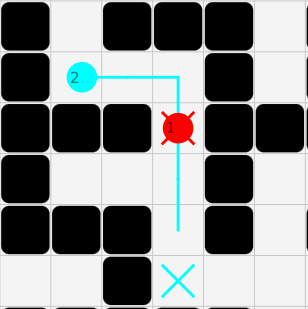
\includegraphics[width=0.3\columnwidth]{img/robopath/whca-giveway-1}}
		\qquad
		\subfloat[]{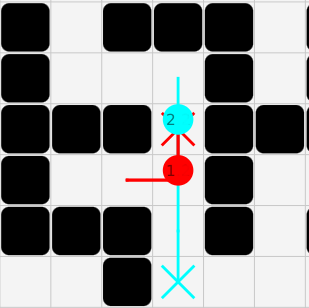
\includegraphics[width=0.3\columnwidth]{img/robopath/whca-giveway-2}}
		\qquad
		\subfloat[]{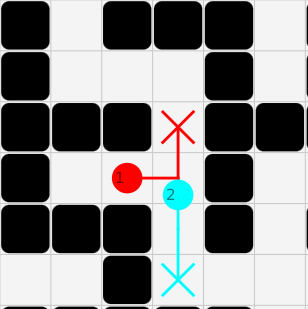
\includegraphics[width=0.3\columnwidth]{img/robopath/whca-giveway-3}}
	\caption{Przykładowa sytuacja "przepuszczania się" robotów uzyskana metodą WHCA*1:
	(a) Wyznaczona trasa przez robota 2 koliduje z aktualnym położeniem robota 1, który dotarł już do celu.
	(b) Robot 1 schodzi z drogi robotowi 2, ukrywając się we "wnęce".
	(c) Robot 2 może bezkolizyjnie dotrzeć do celu. Następnie robot 1 może powrócić do celu.}
	\label{fig:whca-giveway}
\end{figure}
% Wstępne obserwacje pozwalają stwierdzić, że algorytm radzi sobie stosunkowo dobrze nawet na mapach z wąkimi gardłami i dużą liczbą robotów.

Obszerne testy skuteczności oraz innych wskaźników zaprojektowanej metody WHCA*1 zostały opisane dokładniej w dalszym rozdziale \ref{ch:tests}.
% TODO screen jak schodzą sobie z drogi z zaznaczeniem tras (kolejne screeny)

Wadą i ograniczeniem metody jest niezmieniający się przydział priorytetów robotów oraz stała szerokość okna czasowego.
W kolejnej części pokażemy, że dopiero wprowadzenie dynamicznego przydzielania priorytetów oraz skalowania okna czasowego, pozwoliło jeszcze skuteczniej rozwiązywać skomplikowane problemy zakleszczenia robotów.
